\begin{figure}[htbp]
\section*{ SPTAN1 (Part 1/2)}
\centering
\begin{subfigure}[b]{0.95\textwidth}
\centering
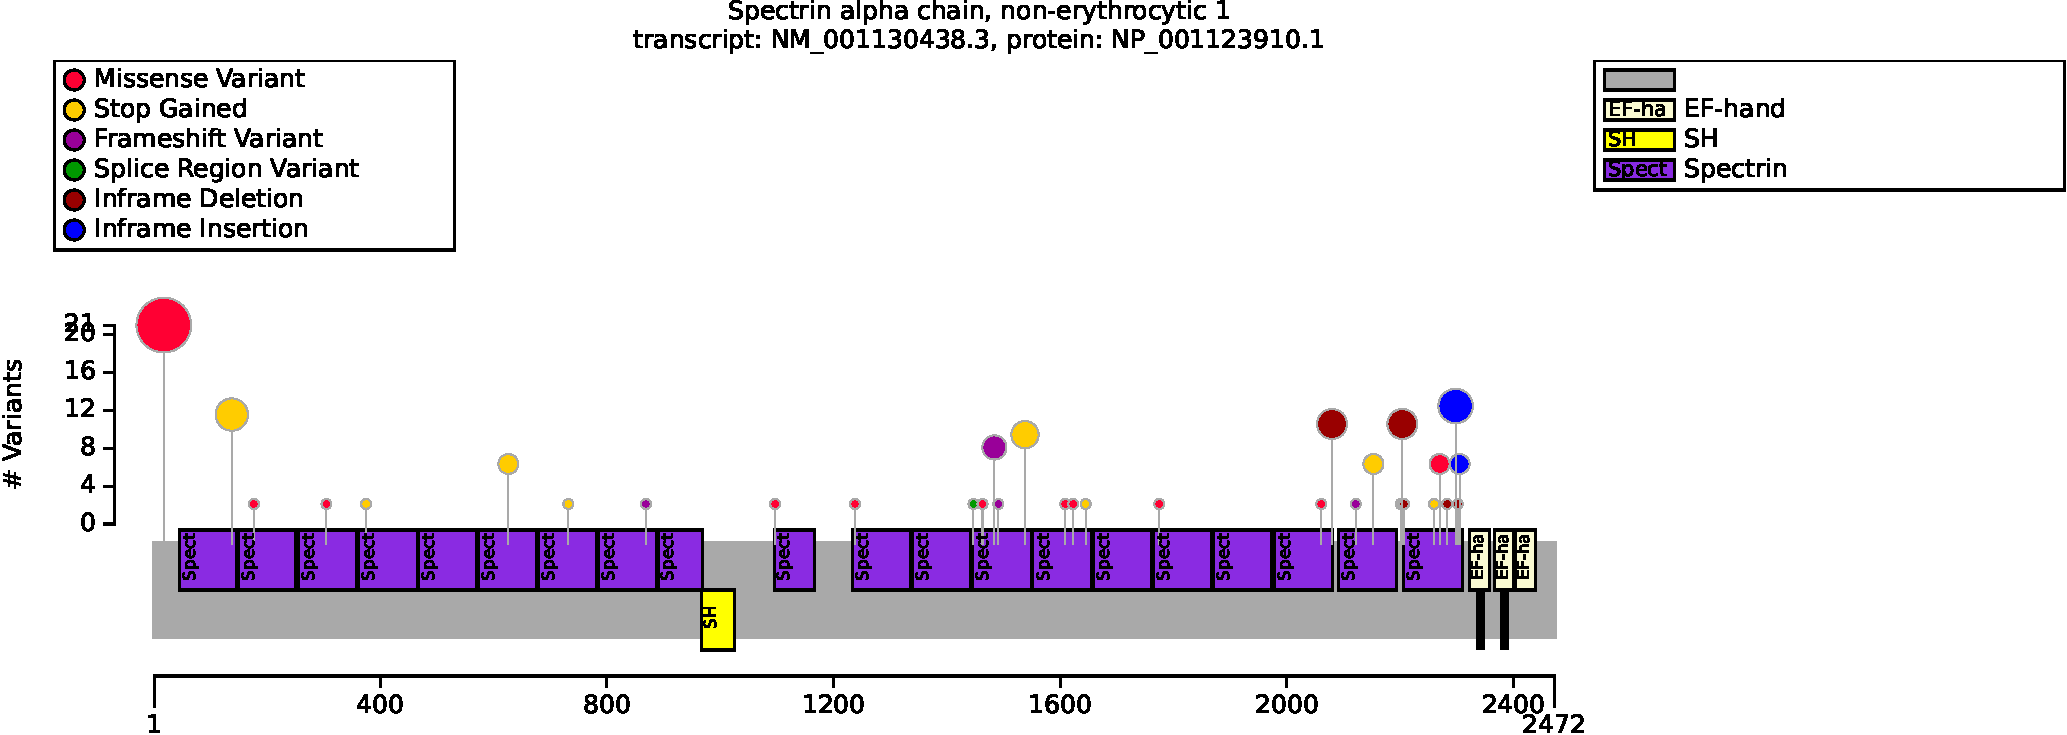
\includegraphics[width=\textwidth]{ img/SPTAN1_protein_diagram.pdf} 
\captionsetup{justification=raggedright,singlelinecheck=false}
\caption{Distribution of variants in SPTAN1}
\end{subfigure}

\vspace{2em}

\begin{subfigure}[b]{0.95\textwidth}
\centering
\resizebox{\textwidth}{!}{
\begin{tabular}{llllrr}
\toprule
HPO term & missense & other & p-value & adj. p-value\\
\midrule
Spastic paraplegia [HP:0001258] & 21/25 (84\%) & 0/16 (0\%) & $4.70\times 10^{-8}$ & $4.70\times 10^{-7}$\\
Lower limb spasticity [HP:0002061] & 21/22 (95\%) & 0/12 (0\%) & $2.37\times 10^{-8}$ & $4.70\times 10^{-7}$\\
Appendicular spasticity [HP:0034353] & 21/22 (95\%) & 2/14 (14\%) & $8.72\times 10^{-7}$ & $5.82\times 10^{-6}$\\
Spasticity [HP:0001257] & 22/23 (96\%) & 4/16 (25\%) & $5.22\times 10^{-6}$ & $2.09\times 10^{-5}$\\
Motor axonal neuropathy [HP:0007002] & 0/19 (0\%) & 12/16 (75\%) & $2.18\times 10^{-6}$ & $1.09\times 10^{-5}$\\
Epileptic spasm [HP:0011097] & 2/22 (9\%) & 13/17 (76\%) & $2.93\times 10^{-5}$ & $9.75\times 10^{-5}$\\
Peripheral axonal neuropathy [HP:0003477] & 4/23 (17\%) & 12/16 (75\%) & $6.69\times 10^{-4}$ & 0.001\\
Seizure [HP:0001250] & 13/33 (39\%) & 24/28 (86\%) & $2.48\times 10^{-4}$ & $7.09\times 10^{-4}$\\
Intellectual disability [HP:0001249] & 9/32 (28\%) & 18/23 (78\%) & $3.43\times 10^{-4}$ & $8.57\times 10^{-4}$\\
Distal lower limb muscle weakness [HP:0009053] & 9/19 (47\%) & 0/16 (0\%) & 0.001 & 0.003\\
Infantile spasms [HP:0012469] & 2/29 (7\%) & 13/31 (42\%) & 0.002 & 0.004\\
Motor seizure [HP:0020219] & 7/27 (26\%) & 13/17 (76\%) & 0.002 & 0.003\\
Microcephaly [HP:0000252] & 4/34 (12\%) & 15/32 (47\%) & 0.002 & 0.004\\
Lower limb muscle weakness [HP:0007340] & 15/16 (94\%) & 16/28 (57\%) & 0.015 & 0.022\\
\bottomrule
\end{tabular}
}
\captionsetup{justification=raggedright,singlelinecheck=false}
\caption{Fisher Exact Test performed to compare HPO annotation frequency with respect to missense and other. Total of
        20 tests were performed.}
\end{subfigure}
\vspace{2em}
\begin{subfigure}[b]{0.95\textwidth}
\centering
\resizebox{\textwidth}{!}{
\begin{tabular}{llllrr}
\toprule
HPO term & truncating & other & p-value & adj. p-value\\
\midrule
Motor axonal neuropathy [HP:0007002] & 12/12 (100\%) & 0/23 (0\%) & $1.20\times 10^{-9}$ & $1.80\times 10^{-8}$\\
Peripheral axonal neuropathy [HP:0003477] & 12/12 (100\%) & 4/27 (15\%) & $4.65\times 10^{-7}$ & $3.49\times 10^{-6}$\\
Spasticity [HP:0001257] & 0/8 (0\%) & 26/31 (84\%) & $2.09\times 10^{-5}$ & $1.05\times 10^{-4}$\\
Appendicular spasticity [HP:0034353] & 0/8 (0\%) & 23/28 (82\%) & $4.25\times 10^{-5}$ & $1.59\times 10^{-4}$\\
Lower limb spasticity [HP:0002061] & 0/8 (0\%) & 21/26 (81\%) & $7.09\times 10^{-5}$ & $2.13\times 10^{-4}$\\
Spastic paraplegia [HP:0001258] & 0/8 (0\%) & 21/33 (64\%) & 0.001 & 0.003\\
Hypotonia [HP:0001252] & 1/11 (9\%) & 15/24 (62\%) & 0.004 & 0.009\\
\bottomrule
\end{tabular}
}
\captionsetup{justification=raggedright,singlelinecheck=false}
\caption{Fisher Exact Test performed to compare HPO annotation frequency with respect to truncating and other. Total of
        15 tests were performed. }
\end{subfigure}
\caption{See next page for caption}
\end{figure}

\begin{figure}[htbp]
\section*{ SPTAN1 (Part 2/2)}

\begin{subfigure}[b]{0.95\textwidth}
\centering
\resizebox{\textwidth}{!}{
\begin{tabular}{llllrr}
\toprule
HPO term & Arg19Trp & Other & p-value & adj. p-value\\
\midrule
Spastic paraplegia [HP:0001258] & 21/21 (100\%) & 0/20 (0\%) & $3.72\times 10^{-12}$ & $5.95\times 10^{-11}$\\
Lower limb spasticity [HP:0002061] & 21/21 (100\%) & 0/13 (0\%) & $1.08\times 10^{-9}$ & $8.62\times 10^{-9}$\\
Appendicular spasticity [HP:0034353] & 21/21 (100\%) & 2/15 (13\%) & $4.54\times 10^{-8}$ & $1.21\times 10^{-7}$\\
Spasticity [HP:0001257] & 21/21 (100\%) & 5/18 (28\%) & $1.05\times 10^{-6}$ & $2.11\times 10^{-6}$\\
Motor axonal neuropathy [HP:0007002] & 0/16 (0\%) & 12/19 (63\%) & $6.26\times 10^{-5}$ & $1.11\times 10^{-4}$\\
Peripheral axonal neuropathy [HP:0003477] & 4/20 (20\%) & 12/19 (63\%) & 0.010 & 0.012\\
Motor seizure [HP:0020219] & 0/19 (0\%) & 20/25 (80\%) & $3.34\times 10^{-8}$ & $1.07\times 10^{-7}$\\
Seizure [HP:0001250] & 2/21 (10\%) & 35/40 (88\%) & $2.36\times 10^{-9}$ & $9.43\times 10^{-9}$\\
Intellectual disability [HP:0001249] & 0/21 (0\%) & 27/34 (79\%) & $1.76\times 10^{-9}$ & $9.38\times 10^{-9}$\\
Lower limb muscle weakness [HP:0007340] & 14/14 (100\%) & 17/30 (57\%) & 0.003 & 0.005\\
Distal lower limb muscle weakness [HP:0009053] & 8/15 (53\%) & 1/20 (5\%) & 0.002 & 0.003\\
Epileptic spasm [HP:0011097] & 0/19 (0\%) & 15/20 (75\%) & $7.71\times 10^{-7}$ & $1.76\times 10^{-6}$\\
Microcephaly [HP:0000252] & 0/21 (0\%) & 19/45 (42\%) & $2.45\times 10^{-4}$ & $3.93\times 10^{-4}$\\
\bottomrule
\end{tabular}
}
\captionsetup{justification=raggedright,singlelinecheck=false}
\caption{Fisher Exact Test performed to compare HPO annotation frequency with respect to Arg19Trp and Other. Total of
        16 tests were performed. }
\end{subfigure}
\vspace{2em}
\begin{subfigure}[b]{0.95\textwidth}
\centering
\resizebox{\textwidth}{!}{
\begin{tabular}{llllrr}
\toprule
Genotype (A) & Genotype (B) & total tests performed & significant results\\
\midrule
Lys2083del & Other & 9 & 0\\
FEMALE & MALE & 1 & 0\\
\bottomrule
\end{tabular}
}
\captionsetup{justification=raggedright,singlelinecheck=false}
\caption{Fisher Exact Test performed to compare HPO annotation frequency with respect to genotypes. }
\end{subfigure}

\vspace{2em}

\caption{ The cohort comprised 85 individuals (40 females, 45 males). 3 of these individuals were reported to be deceased. A total of 96 HPO terms were used to annotate the cohort. Disease diagnoses: Spastic paraplegia 91, autosomal dominant, with or without cerebellar ataxia (OMIM:620538) (28 individuals), Developmental and epileptic encephalopathy 5 (OMIM:613477) (22 individuals), Developmental delay with or without epilepsy (OMIM:620540) (21 individuals), Neuronopathy, distal hereditary motor, autosomal dominant 11 (OMIM:620528) (14 individuals). Several publications have identified genotype-phenotype correlations in SPTAN1 that are comparable to those
identified here \cite{PMID_25631096,PMID_36331550,PMID_35150594}.
 A total of 85 unique variant alleles were found in \textit{SPTAN1} (transcript: \texttt{NM\_001130438.3}, protein id: \texttt{NP\_001123910.1}).}
\end{figure}
